\documentclass[1p]{elsarticle_modified}
%\bibliographystyle{elsarticle-num}

%\usepackage[colorlinks]{hyperref}
%\usepackage{abbrmath_seonhwa} %\Abb, \Ascr, \Acal ,\Abf, \Afrak
\usepackage{amsfonts}
\usepackage{amssymb}
\usepackage{amsmath}
\usepackage{amsthm}
\usepackage{scalefnt}
\usepackage{amsbsy}
\usepackage{kotex}
\usepackage{caption}
\usepackage{subfig}
\usepackage{color}
\usepackage{graphicx}
\usepackage{xcolor} %% white, black, red, green, blue, cyan, magenta, yellow
\usepackage{float}
\usepackage{setspace}
\usepackage{hyperref}

\usepackage{tikz}
\usetikzlibrary{arrows}

\usepackage{multirow}
\usepackage{array} % fixed length table
\usepackage{hhline}

%%%%%%%%%%%%%%%%%%%%%
\makeatletter
\renewcommand*\env@matrix[1][\arraystretch]{%
	\edef\arraystretch{#1}%
	\hskip -\arraycolsep
	\let\@ifnextchar\new@ifnextchar
	\array{*\c@MaxMatrixCols c}}
\makeatother %https://tex.stackexchange.com/questions/14071/how-can-i-increase-the-line-spacing-in-a-matrix
%%%%%%%%%%%%%%%

\usepackage[normalem]{ulem}

\newcommand{\msout}[1]{\ifmmode\text{\sout{\ensuremath{#1}}}\else\sout{#1}\fi}
%SOURCE: \msout is \stkout macro in https://tex.stackexchange.com/questions/20609/strikeout-in-math-mode

\newcommand{\cancel}[1]{
	\ifmmode
	{\color{red}\msout{#1}}
	\else
	{\color{red}\sout{#1}}
	\fi
}

\newcommand{\add}[1]{
	{\color{blue}\uwave{#1}}
}

\newcommand{\replace}[2]{
	\ifmmode
	{\color{red}\msout{#1}}{\color{blue}\uwave{#2}}
	\else
	{\color{red}\sout{#1}}{\color{blue}\uwave{#2}}
	\fi
}

\newcommand{\Sol}{\mathcal{S}} %segment
\newcommand{\D}{D} %diagram
\newcommand{\A}{\mathcal{A}} %arc


%%%%%%%%%%%%%%%%%%%%%%%%%%%%%5 test

\def\sl{\operatorname{\textup{SL}}(2,\Cbb)}
\def\psl{\operatorname{\textup{PSL}}(2,\Cbb)}
\def\quan{\mkern 1mu \triangleright \mkern 1mu}

\theoremstyle{definition}
\newtheorem{thm}{Theorem}[section]
\newtheorem{prop}[thm]{Proposition}
\newtheorem{lem}[thm]{Lemma}
\newtheorem{ques}[thm]{Question}
\newtheorem{cor}[thm]{Corollary}
\newtheorem{defn}[thm]{Definition}
\newtheorem{exam}[thm]{Example}
\newtheorem{rmk}[thm]{Remark}
\newtheorem{alg}[thm]{Algorithm}

\newcommand{\I}{\sqrt{-1}}
\begin{document}

%\begin{frontmatter}
%
%\title{Boundary parabolic representations of knots up to 8 crossings}
%
%%% Group authors per affiliation:
%\author{Yunhi Cho} 
%\address{Department of Mathematics, University of Seoul, Seoul, Korea}
%\ead{yhcho@uos.ac.kr}
%
%
%\author{Seonhwa Kim} %\fnref{s_kim}}
%\address{Center for Geometry and Physics, Institute for Basic Science, Pohang, 37673, Korea}
%\ead{ryeona17@ibs.re.kr}
%
%\author{Hyuk Kim}
%\address{Department of Mathematical Sciences, Seoul National University, Seoul 08826, Korea}
%\ead{hyukkim@snu.ac.kr}
%
%\author{Seokbeom Yoon}
%\address{Department of Mathematical Sciences, Seoul National University, Seoul, 08826,  Korea}
%\ead{sbyoon15@snu.ac.kr}
%
%\begin{abstract}
%We find all boundary parabolic representation of knots up to 8 crossings.
%
%\end{abstract}
%\begin{keyword}
%    \MSC[2010] 57M25 
%\end{keyword}
%
%\end{frontmatter}

%\linenumbers
%\tableofcontents
%
\newcommand\colored[1]{\textcolor{white}{\rule[-0.35ex]{0.8em}{1.4ex}}\kern-0.8em\color{red} #1}%
%\newcommand\colored[1]{\textcolor{white}{ #1}\kern-2.17ex	\textcolor{white}{ #1}\kern-1.81ex	\textcolor{white}{ #1}\kern-2.15ex\color{red}#1	}

{\Large $\underline{12a_{0565}~(K12a_{0565})}$}

\setlength{\tabcolsep}{10pt}
\renewcommand{\arraystretch}{1.6}
\vspace{1cm}\begin{tabular}{m{100pt}>{\centering\arraybackslash}m{274pt}}
\multirow{5}{120pt}{
	\centering
	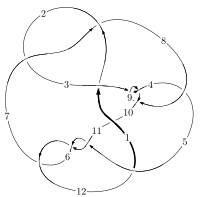
\includegraphics[width=112pt]{../../../GIT/diagram.site/Diagrams/png/1366_12a_0565.png}\\
\ \ \ A knot diagram\footnotemark}&
\allowdisplaybreaks
\textbf{Linearized knot diagam} \\
\cline{2-2}
 &
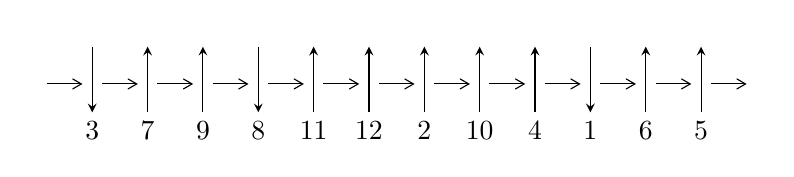
\begin{tikzpicture}[x=20pt, y=17pt]
	% nodes
	\node (C0) at (0, 0) {};
	\node (C1) at (1, 0) {};
	\node (C1U) at (1, +1) {};
	\node (C1D) at (1, -1) {3};

	\node (C2) at (2, 0) {};
	\node (C2U) at (2, +1) {};
	\node (C2D) at (2, -1) {7};

	\node (C3) at (3, 0) {};
	\node (C3U) at (3, +1) {};
	\node (C3D) at (3, -1) {9};

	\node (C4) at (4, 0) {};
	\node (C4U) at (4, +1) {};
	\node (C4D) at (4, -1) {8};

	\node (C5) at (5, 0) {};
	\node (C5U) at (5, +1) {};
	\node (C5D) at (5, -1) {11};

	\node (C6) at (6, 0) {};
	\node (C6U) at (6, +1) {};
	\node (C6D) at (6, -1) {12};

	\node (C7) at (7, 0) {};
	\node (C7U) at (7, +1) {};
	\node (C7D) at (7, -1) {2};

	\node (C8) at (8, 0) {};
	\node (C8U) at (8, +1) {};
	\node (C8D) at (8, -1) {10};

	\node (C9) at (9, 0) {};
	\node (C9U) at (9, +1) {};
	\node (C9D) at (9, -1) {4};

	\node (C10) at (10, 0) {};
	\node (C10U) at (10, +1) {};
	\node (C10D) at (10, -1) {1};

	\node (C11) at (11, 0) {};
	\node (C11U) at (11, +1) {};
	\node (C11D) at (11, -1) {6};

	\node (C12) at (12, 0) {};
	\node (C12U) at (12, +1) {};
	\node (C12D) at (12, -1) {5};
	\node (C13) at (13, 0) {};

	% arrows
	\draw[->,>={angle 60}]
	(C0) edge (C1) (C1) edge (C2) (C2) edge (C3) (C3) edge (C4) (C4) edge (C5) (C5) edge (C6) (C6) edge (C7) (C7) edge (C8) (C8) edge (C9) (C9) edge (C10) (C10) edge (C11) (C11) edge (C12) (C12) edge (C13) ;	\draw[->,>=stealth]
	(C1U) edge (C1D) (C2D) edge (C2U) (C3D) edge (C3U) (C4U) edge (C4D) (C5D) edge (C5U) (C6D) edge (C6U) (C7D) edge (C7U) (C8D) edge (C8U) (C9D) edge (C9U) (C10U) edge (C10D) (C11D) edge (C11U) (C12D) edge (C12U) ;
	\end{tikzpicture} \\
\hhline{~~} \\& 
\textbf{Solving Sequence} \\ \cline{2-2} 
 &
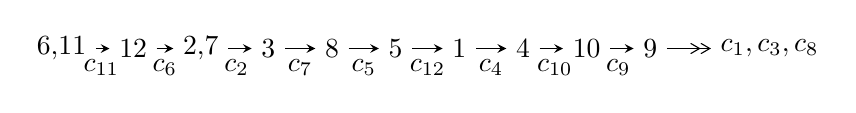
\begin{tikzpicture}[x=23pt, y=7pt]
	% node
	\node (A0) at (-1/8, 0) {6,11};
	\node (A1) at (1, 0) {12};
	\node (A2) at (33/16, 0) {2,7};
	\node (A3) at (25/8, 0) {3};
	\node (A4) at (33/8, 0) {8};
	\node (A5) at (41/8, 0) {5};
	\node (A6) at (49/8, 0) {1};
	\node (A7) at (57/8, 0) {4};
	\node (A8) at (65/8, 0) {10};
	\node (A9) at (73/8, 0) {9};
	\node (C1) at (1/2, -1) {$c_{11}$};
	\node (C2) at (3/2, -1) {$c_{6}$};
	\node (C3) at (21/8, -1) {$c_{2}$};
	\node (C4) at (29/8, -1) {$c_{7}$};
	\node (C5) at (37/8, -1) {$c_{5}$};
	\node (C6) at (45/8, -1) {$c_{12}$};
	\node (C7) at (53/8, -1) {$c_{4}$};
	\node (C8) at (61/8, -1) {$c_{10}$};
	\node (C9) at (69/8, -1) {$c_{9}$};
	\node (A10) at (11, 0) {$c_{1},c_{3},c_{8}$};

	% edge
	\draw[->,>=stealth]	
	(A0) edge (A1) (A1) edge (A2) (A2) edge (A3) (A3) edge (A4) (A4) edge (A5) (A5) edge (A6) (A6) edge (A7) (A7) edge (A8) (A8) edge (A9) ;
	\draw[->>,>={angle 60}]	
	(A9) edge (A10);
\end{tikzpicture} \\ 

\end{tabular} \\

\footnotetext{
The image of knot diagram is generated by the software ``\textbf{Draw programme}" developed by Andrew Bartholomew(\url{http://www.layer8.co.uk/maths/draw/index.htm\#Running-draw}), where we modified some parts for our purpose(\url{https://github.com/CATsTAILs/LinksPainter}).
}\phantom \\ \newline 
\centering \textbf{Ideals for irreducible components\footnotemark of $X_{\text{par}}$} 
 
\begin{align*}
I^u_{1}&=\langle 
1.32158\times10^{56} u^{107}+3.27224\times10^{55} u^{106}+\cdots+4.96026\times10^{55} b-4.27420\times10^{55},\\
\phantom{I^u_{1}}&\phantom{= \langle  }-1.26324\times10^{55} u^{107}-5.20004\times10^{54} u^{106}+\cdots+4.96026\times10^{55} a+2.69630\times10^{55},\;u^{108}+u^{107}+\cdots+4 u-1\rangle \\
I^u_{2}&=\langle 
- u^4+u^2 a+2 u^2+b- a-1,\;4 u^4 a+u^5+u^3 a-2 u^4-6 u^2 a-2 u^3+a^2- a u+u^2-2 a- u,\\
\phantom{I^u_{2}}&\phantom{= \langle  }u^6-3 u^4+2 u^2+1\rangle \\
\\
\end{align*}
\raggedright * 2 irreducible components of $\dim_{\mathbb{C}}=0$, with total 120 representations.\\
\footnotetext{All coefficients of polynomials are rational numbers. But the coefficients are sometimes approximated in decimal forms when there is not enough margin.}
\newpage
\renewcommand{\arraystretch}{1}
\centering \section*{I. $I^u_{1}= \langle 1.32\times10^{56} u^{107}+3.27\times10^{55} u^{106}+\cdots+4.96\times10^{55} b-4.27\times10^{55},\;-1.26\times10^{55} u^{107}-5.20\times10^{54} u^{106}+\cdots+4.96\times10^{55} a+2.70\times10^{55},\;u^{108}+u^{107}+\cdots+4 u-1 \rangle$}
\flushleft \textbf{(i) Arc colorings}\\
\begin{tabular}{m{7pt} m{180pt} m{7pt} m{180pt} }
\flushright $a_{6}=$&$\begin{pmatrix}0\\u\end{pmatrix}$ \\
\flushright $a_{11}=$&$\begin{pmatrix}1\\0\end{pmatrix}$ \\
\flushright $a_{12}=$&$\begin{pmatrix}1\\- u^2\end{pmatrix}$ \\
\flushright $a_{2}=$&$\begin{pmatrix}0.254671 u^{107}+0.104834 u^{106}+\cdots+14.4074 u-0.543580\\-2.66434 u^{107}-0.659690 u^{106}+\cdots-2.76765 u+0.861688\end{pmatrix}$ \\
\flushright $a_{7}=$&$\begin{pmatrix}u\\- u^3+u\end{pmatrix}$ \\
\flushright $a_{3}=$&$\begin{pmatrix}-0.915359 u^{107}-1.08630 u^{106}+\cdots+14.1070 u-0.0176901\\-1.60412 u^{107}-0.998446 u^{106}+\cdots-1.98244 u+1.40868\end{pmatrix}$ \\
\flushright $a_{8}=$&$\begin{pmatrix}-1.55496 u^{107}-1.18445 u^{106}+\cdots+10.3009 u-2.64846\\-0.0712391 u^{107}-0.373281 u^{106}+\cdots+10.1195 u-2.22072\end{pmatrix}$ \\
\flushright $a_{5}=$&$\begin{pmatrix}- u\\u\end{pmatrix}$ \\
\flushright $a_{1}=$&$\begin{pmatrix}- u^4+u^2+1\\u^4-2 u^2\end{pmatrix}$ \\
\flushright $a_{4}=$&$\begin{pmatrix}0.557394 u^{107}+0.518033 u^{106}+\cdots-21.2085 u+4.62222\\3.34901 u^{107}+0.543398 u^{106}+\cdots-5.93596 u+1.29539\end{pmatrix}$ \\
\flushright $a_{10}=$&$\begin{pmatrix}u^8-3 u^6+u^4+2 u^2+1\\- u^8+4 u^6-4 u^4\end{pmatrix}$ \\
\flushright $a_{9}=$&$\begin{pmatrix}-1.38003 u^{107}+0.953232 u^{106}+\cdots+9.29014 u-2.70352\\-0.149367 u^{107}-1.02014 u^{106}+\cdots+12.1445 u-2.89736\end{pmatrix}$\\&\end{tabular}
\flushleft \textbf{(ii) Obstruction class $= -1$}\\~\\
\flushleft \textbf{(iii) Cusp Shapes $= 0.876716 u^{107}+1.14842 u^{106}+\cdots-33.0770 u+17.3306$}\\~\\
\newpage\renewcommand{\arraystretch}{1}
\flushleft \textbf{(iv) u-Polynomials at the component}\newline \\
\begin{tabular}{m{50pt}|m{274pt}}
Crossings & \hspace{64pt}u-Polynomials at each crossing \\
\hline $$\begin{aligned}c_{1}\end{aligned}$$&$\begin{aligned}
&u^{108}+53 u^{107}+\cdots+24 u+1
\end{aligned}$\\
\hline $$\begin{aligned}c_{2},c_{7}\end{aligned}$$&$\begin{aligned}
&u^{108}+u^{107}+\cdots-6 u-1
\end{aligned}$\\
\hline $$\begin{aligned}c_{3},c_{9}\end{aligned}$$&$\begin{aligned}
&u^{108}+u^{107}+\cdots+21 u^2-5
\end{aligned}$\\
\hline $$\begin{aligned}c_{4}\end{aligned}$$&$\begin{aligned}
&u^{108}+3 u^{107}+\cdots-461530 u-25545
\end{aligned}$\\
\hline $$\begin{aligned}c_{5},c_{6},c_{11}\end{aligned}$$&$\begin{aligned}
&u^{108}+u^{107}+\cdots+4 u-1
\end{aligned}$\\
\hline $$\begin{aligned}c_{8}\end{aligned}$$&$\begin{aligned}
&u^{108}-53 u^{107}+\cdots-210 u+25
\end{aligned}$\\
\hline $$\begin{aligned}c_{10}\end{aligned}$$&$\begin{aligned}
&u^{108}-23 u^{107}+\cdots-841432 u+42793
\end{aligned}$\\
\hline $$\begin{aligned}c_{12}\end{aligned}$$&$\begin{aligned}
&u^{108}-3 u^{107}+\cdots-334 u+99
\end{aligned}$\\
\hline
\end{tabular}\\~\\
\newpage\renewcommand{\arraystretch}{1}
\flushleft \textbf{(v) Riley Polynomials at the component}\newline \\
\begin{tabular}{m{50pt}|m{274pt}}
Crossings & \hspace{64pt}Riley Polynomials at each crossing \\
\hline $$\begin{aligned}c_{1}\end{aligned}$$&$\begin{aligned}
&y^{108}+17 y^{107}+\cdots-324 y+1
\end{aligned}$\\
\hline $$\begin{aligned}c_{2},c_{7}\end{aligned}$$&$\begin{aligned}
&y^{108}+53 y^{107}+\cdots+24 y+1
\end{aligned}$\\
\hline $$\begin{aligned}c_{3},c_{9}\end{aligned}$$&$\begin{aligned}
&y^{108}-53 y^{107}+\cdots-210 y+25
\end{aligned}$\\
\hline $$\begin{aligned}c_{4}\end{aligned}$$&$\begin{aligned}
&y^{108}+31 y^{107}+\cdots-307924380910 y+652547025
\end{aligned}$\\
\hline $$\begin{aligned}c_{5},c_{6},c_{11}\end{aligned}$$&$\begin{aligned}
&y^{108}-99 y^{107}+\cdots+4 y+1
\end{aligned}$\\
\hline $$\begin{aligned}c_{8}\end{aligned}$$&$\begin{aligned}
&y^{108}+11 y^{107}+\cdots+17950 y+625
\end{aligned}$\\
\hline $$\begin{aligned}c_{10}\end{aligned}$$&$\begin{aligned}
&y^{108}+37 y^{107}+\cdots+17887794312 y+1831240849
\end{aligned}$\\
\hline $$\begin{aligned}c_{12}\end{aligned}$$&$\begin{aligned}
&y^{108}-7 y^{107}+\cdots-323416 y+9801
\end{aligned}$\\
\hline
\end{tabular}\\~\\
\newpage\flushleft \textbf{(vi) Complex Volumes and Cusp Shapes}
$$\begin{array}{c|c|c}  
\text{Solutions to }I^u_{1}& \I (\text{vol} + \sqrt{-1}CS) & \text{Cusp shape}\\
 \hline 
\begin{aligned}
u &= -1.078510 + 0.066384 I \\
a &= \phantom{-}0.74913 + 2.91711 I \\
b &= -0.159122 - 1.375640 I\end{aligned}
 & -1.75904 - 2.65358 I & \phantom{-0.000000 } 0 \\ \hline\begin{aligned}
u &= -1.078510 - 0.066384 I \\
a &= \phantom{-}0.74913 - 2.91711 I \\
b &= -0.159122 + 1.375640 I\end{aligned}
 & -1.75904 + 2.65358 I & \phantom{-0.000000 } 0 \\ \hline\begin{aligned}
u &= -1.091430 + 0.244782 I \\
a &= \phantom{-}0.49231 + 2.62431 I \\
b &= -0.860462 - 0.916898 I\end{aligned}
 & -0.96511 - 4.47596 I & \phantom{-0.000000 } 0 \\ \hline\begin{aligned}
u &= -1.091430 - 0.244782 I \\
a &= \phantom{-}0.49231 - 2.62431 I \\
b &= -0.860462 + 0.916898 I\end{aligned}
 & -0.96511 + 4.47596 I & \phantom{-0.000000 } 0 \\ \hline\begin{aligned}
u &= \phantom{-}1.133480 + 0.015855 I \\
a &= \phantom{-}1.05659 + 3.14794 I \\
b &= \phantom{-}0.06419 - 1.93882 I\end{aligned}
 & -0.45128 + 2.17405 I & \phantom{-0.000000 } 0 \\ \hline\begin{aligned}
u &= \phantom{-}1.133480 - 0.015855 I \\
a &= \phantom{-}1.05659 - 3.14794 I \\
b &= \phantom{-}0.06419 + 1.93882 I\end{aligned}
 & -0.45128 - 2.17405 I & \phantom{-0.000000 } 0 \\ \hline\begin{aligned}
u &= \phantom{-}1.099430 + 0.302544 I \\
a &= \phantom{-}0.38080 - 2.61193 I \\
b &= -1.083300 + 0.814934 I\end{aligned}
 & \phantom{-}1.19055 + 9.20491 I & \phantom{-0.000000 } 0 \\ \hline\begin{aligned}
u &= \phantom{-}1.099430 - 0.302544 I \\
a &= \phantom{-}0.38080 + 2.61193 I \\
b &= -1.083300 - 0.814934 I\end{aligned}
 & \phantom{-}1.19055 - 9.20491 I & \phantom{-0.000000 } 0 \\ \hline\begin{aligned}
u &= \phantom{-}1.164780 + 0.108311 I \\
a &= \phantom{-}0.637076 - 0.329305 I \\
b &= -0.785331 + 0.058134 I\end{aligned}
 & \phantom{-}1.56546 + 0.67321 I & \phantom{-0.000000 } 0 \\ \hline\begin{aligned}
u &= \phantom{-}1.164780 - 0.108311 I \\
a &= \phantom{-}0.637076 + 0.329305 I \\
b &= -0.785331 - 0.058134 I\end{aligned}
 & \phantom{-}1.56546 - 0.67321 I & \phantom{-0.000000 } 0\\
 \hline 
 \end{array}$$\newpage$$\begin{array}{c|c|c}  
\text{Solutions to }I^u_{1}& \I (\text{vol} + \sqrt{-1}CS) & \text{Cusp shape}\\
 \hline 
\begin{aligned}
u &= \phantom{-}0.691156 + 0.445702 I \\
a &= -0.57421 + 2.25405 I \\
b &= \phantom{-}0.881318 + 0.430710 I\end{aligned}
 & \phantom{-}2.28872 - 9.22034 I & \phantom{-}8.40055 + 5.38134 I \\ \hline\begin{aligned}
u &= \phantom{-}0.691156 - 0.445702 I \\
a &= -0.57421 - 2.25405 I \\
b &= \phantom{-}0.881318 - 0.430710 I\end{aligned}
 & \phantom{-}2.28872 + 9.22034 I & \phantom{-}8.40055 - 5.38134 I \\ \hline\begin{aligned}
u &= \phantom{-}0.312027 + 0.742416 I \\
a &= -0.599810 - 0.003658 I \\
b &= -2.50501 + 0.43469 I\end{aligned}
 & \phantom{-}0.94501 + 13.40950 I & \phantom{-}5.88106 - 10.27839 I \\ \hline\begin{aligned}
u &= \phantom{-}0.312027 - 0.742416 I \\
a &= -0.599810 + 0.003658 I \\
b &= -2.50501 - 0.43469 I\end{aligned}
 & \phantom{-}0.94501 - 13.40950 I & \phantom{-}5.88106 + 10.27839 I \\ \hline\begin{aligned}
u &= -0.304870 + 0.721074 I \\
a &= -0.533307 + 0.121712 I \\
b &= -2.43367 - 0.20539 I\end{aligned}
 & -1.48238 - 8.19805 I & \phantom{-}2.90543 + 6.87933 I \\ \hline\begin{aligned}
u &= -0.304870 - 0.721074 I \\
a &= -0.533307 - 0.121712 I \\
b &= -2.43367 + 0.20539 I\end{aligned}
 & -1.48238 + 8.19805 I & \phantom{-}2.90543 - 6.87933 I \\ \hline\begin{aligned}
u &= \phantom{-}0.345057 + 0.699162 I \\
a &= -0.286884 - 0.018001 I \\
b &= -1.97972 + 0.27664 I\end{aligned}
 & \phantom{-}3.40555 + 5.22912 I & \phantom{-}9.21272 - 5.28491 I \\ \hline\begin{aligned}
u &= \phantom{-}0.345057 - 0.699162 I \\
a &= -0.286884 + 0.018001 I \\
b &= -1.97972 - 0.27664 I\end{aligned}
 & \phantom{-}3.40555 - 5.22912 I & \phantom{-}9.21272 + 5.28491 I \\ \hline\begin{aligned}
u &= -0.338529 + 0.700114 I \\
a &= -0.176477 - 0.453278 I \\
b &= \phantom{-}0.044291 + 0.534112 I\end{aligned}
 & \phantom{-}3.32780 - 7.81069 I & \phantom{-}9.09509 + 6.82204 I \\ \hline\begin{aligned}
u &= -0.338529 - 0.700114 I \\
a &= -0.176477 + 0.453278 I \\
b &= \phantom{-}0.044291 - 0.534112 I\end{aligned}
 & \phantom{-}3.32780 + 7.81069 I & \phantom{-}9.09509 - 6.82204 I\\
 \hline 
 \end{array}$$\newpage$$\begin{array}{c|c|c}  
\text{Solutions to }I^u_{1}& \I (\text{vol} + \sqrt{-1}CS) & \text{Cusp shape}\\
 \hline 
\begin{aligned}
u &= -0.651351 + 0.404173 I \\
a &= -0.34954 - 2.24628 I \\
b &= \phantom{-}0.828682 - 0.267745 I\end{aligned}
 & -0.17377 + 4.20459 I & \phantom{-}5.40595 - 1.84900 I \\ \hline\begin{aligned}
u &= -0.651351 - 0.404173 I \\
a &= -0.34954 + 2.24628 I \\
b &= \phantom{-}0.828682 + 0.267745 I\end{aligned}
 & -0.17377 - 4.20459 I & \phantom{-}5.40595 + 1.84900 I \\ \hline\begin{aligned}
u &= \phantom{-}0.098301 + 0.756192 I \\
a &= \phantom{-}0.582497 - 0.315067 I \\
b &= \phantom{-}2.05472 + 0.23854 I\end{aligned}
 & -1.85912 - 5.30654 I & \phantom{-}4.29467 + 5.82125 I \\ \hline\begin{aligned}
u &= \phantom{-}0.098301 - 0.756192 I \\
a &= \phantom{-}0.582497 + 0.315067 I \\
b &= \phantom{-}2.05472 - 0.23854 I\end{aligned}
 & -1.85912 + 5.30654 I & \phantom{-}4.29467 - 5.82125 I \\ \hline\begin{aligned}
u &= \phantom{-}1.209590 + 0.269103 I \\
a &= \phantom{-}0.44287 - 2.25971 I \\
b &= -1.16164 + 1.17315 I\end{aligned}
 & \phantom{-}2.86997 + 2.24160 I & \phantom{-0.000000 } 0 \\ \hline\begin{aligned}
u &= \phantom{-}1.209590 - 0.269103 I \\
a &= \phantom{-}0.44287 + 2.25971 I \\
b &= -1.16164 - 1.17315 I\end{aligned}
 & \phantom{-}2.86997 - 2.24160 I & \phantom{-0.000000 } 0 \\ \hline\begin{aligned}
u &= \phantom{-}0.583376 + 0.482300 I \\
a &= -0.37395 + 1.83053 I \\
b &= \phantom{-}0.557650 + 0.305960 I\end{aligned}
 & \phantom{-}4.32970 - 1.18610 I & \phantom{-}11.36506 - 0.65831 I \\ \hline\begin{aligned}
u &= \phantom{-}0.583376 - 0.482300 I \\
a &= -0.37395 - 1.83053 I \\
b &= \phantom{-}0.557650 - 0.305960 I\end{aligned}
 & \phantom{-}4.32970 + 1.18610 I & \phantom{-}11.36506 + 0.65831 I \\ \hline\begin{aligned}
u &= -0.584735 + 0.471879 I \\
a &= \phantom{-}0.824618 - 0.223152 I \\
b &= -0.381146 + 0.027264 I\end{aligned}
 & \phantom{-}4.29184 + 3.79474 I & \phantom{-}11.40196 - 0.85477 I \\ \hline\begin{aligned}
u &= -0.584735 - 0.471879 I \\
a &= \phantom{-}0.824618 + 0.223152 I \\
b &= -0.381146 - 0.027264 I\end{aligned}
 & \phantom{-}4.29184 - 3.79474 I & \phantom{-}11.40196 + 0.85477 I\\
 \hline 
 \end{array}$$\newpage$$\begin{array}{c|c|c}  
\text{Solutions to }I^u_{1}& \I (\text{vol} + \sqrt{-1}CS) & \text{Cusp shape}\\
 \hline 
\begin{aligned}
u &= -0.395123 + 0.635568 I \\
a &= -0.198792 - 0.793432 I \\
b &= \phantom{-}0.094136 + 0.219436 I\end{aligned}
 & \phantom{-}4.88640 + 0.26560 I & \phantom{-}11.56392 + 0.30422 I \\ \hline\begin{aligned}
u &= -0.395123 - 0.635568 I \\
a &= -0.198792 + 0.793432 I \\
b &= \phantom{-}0.094136 - 0.219436 I\end{aligned}
 & \phantom{-}4.88640 - 0.26560 I & \phantom{-}11.56392 - 0.30422 I \\ \hline\begin{aligned}
u &= -1.229210 + 0.242947 I \\
a &= \phantom{-}0.896086 + 1.028220 I \\
b &= -1.278550 - 0.286411 I\end{aligned}
 & \phantom{-}3.00417 - 4.91856 I & \phantom{-0.000000 } 0 \\ \hline\begin{aligned}
u &= -1.229210 - 0.242947 I \\
a &= \phantom{-}0.896086 - 1.028220 I \\
b &= -1.278550 + 0.286411 I\end{aligned}
 & \phantom{-}3.00417 + 4.91856 I & \phantom{-0.000000 } 0 \\ \hline\begin{aligned}
u &= -0.486434 + 0.557533 I \\
a &= \phantom{-}0.532437 - 0.172628 I \\
b &= -0.699156 - 0.094278 I\end{aligned}
 & \phantom{-}5.23596 - 4.22319 I & \phantom{-}11.96155 + 6.69488 I \\ \hline\begin{aligned}
u &= -0.486434 - 0.557533 I \\
a &= \phantom{-}0.532437 + 0.172628 I \\
b &= -0.699156 + 0.094278 I\end{aligned}
 & \phantom{-}5.23596 + 4.22319 I & \phantom{-}11.96155 - 6.69488 I \\ \hline\begin{aligned}
u &= \phantom{-}0.321740 + 0.658812 I \\
a &= -0.033716 + 0.539334 I \\
b &= \phantom{-}0.190501 - 0.454927 I\end{aligned}
 & \phantom{-}0.71793 + 2.99181 I & \phantom{-}5.99049 - 3.37437 I \\ \hline\begin{aligned}
u &= \phantom{-}0.321740 - 0.658812 I \\
a &= -0.033716 - 0.539334 I \\
b &= \phantom{-}0.190501 + 0.454927 I\end{aligned}
 & \phantom{-}0.71793 - 2.99181 I & \phantom{-}5.99049 + 3.37437 I \\ \hline\begin{aligned}
u &= -0.116202 + 0.710518 I \\
a &= \phantom{-}0.459041 + 0.428398 I \\
b &= \phantom{-}1.92755 - 0.02931 I\end{aligned}
 & -3.89427 + 0.88977 I & -0.482474 - 1.035537 I \\ \hline\begin{aligned}
u &= -0.116202 - 0.710518 I \\
a &= \phantom{-}0.459041 - 0.428398 I \\
b &= \phantom{-}1.92755 + 0.02931 I\end{aligned}
 & -3.89427 - 0.88977 I & -0.482474 + 1.035537 I\\
 \hline 
 \end{array}$$\newpage$$\begin{array}{c|c|c}  
\text{Solutions to }I^u_{1}& \I (\text{vol} + \sqrt{-1}CS) & \text{Cusp shape}\\
 \hline 
\begin{aligned}
u &= \phantom{-}0.010129 + 0.719466 I \\
a &= \phantom{-}0.417716 - 0.122153 I \\
b &= \phantom{-}1.55361 + 0.38676 I\end{aligned}
 & -0.79600 + 1.37844 I & \phantom{-}6.81642 - 0.64656 I \\ \hline\begin{aligned}
u &= \phantom{-}0.010129 - 0.719466 I \\
a &= \phantom{-}0.417716 + 0.122153 I \\
b &= \phantom{-}1.55361 - 0.38676 I\end{aligned}
 & -0.79600 - 1.37844 I & \phantom{-}6.81642 + 0.64656 I \\ \hline\begin{aligned}
u &= -0.263626 + 0.654252 I \\
a &= -0.325800 + 0.611267 I \\
b &= -2.25097 + 0.64555 I\end{aligned}
 & -3.32605 - 5.48665 I & \phantom{-}1.87864 + 8.65808 I \\ \hline\begin{aligned}
u &= -0.263626 - 0.654252 I \\
a &= -0.325800 - 0.611267 I \\
b &= -2.25097 - 0.64555 I\end{aligned}
 & -3.32605 + 5.48665 I & \phantom{-}1.87864 - 8.65808 I \\ \hline\begin{aligned}
u &= -1.280520 + 0.227409 I \\
a &= \phantom{-}0.454469 + 1.305840 I \\
b &= -1.051990 - 0.686908 I\end{aligned}
 & \phantom{-}2.98007 - 4.88539 I & \phantom{-0.000000 } 0 \\ \hline\begin{aligned}
u &= -1.280520 - 0.227409 I \\
a &= \phantom{-}0.454469 - 1.305840 I \\
b &= -1.051990 + 0.686908 I\end{aligned}
 & \phantom{-}2.98007 + 4.88539 I & \phantom{-0.000000 } 0 \\ \hline\begin{aligned}
u &= \phantom{-}1.309160 + 0.119036 I \\
a &= \phantom{-}1.13476 - 2.30065 I \\
b &= -1.28347 + 2.10489 I\end{aligned}
 & \phantom{-}2.32381 + 3.02952 I & \phantom{-0.000000 } 0 \\ \hline\begin{aligned}
u &= \phantom{-}1.309160 - 0.119036 I \\
a &= \phantom{-}1.13476 + 2.30065 I \\
b &= -1.28347 - 2.10489 I\end{aligned}
 & \phantom{-}2.32381 - 3.02952 I & \phantom{-0.000000 } 0 \\ \hline\begin{aligned}
u &= \phantom{-}0.268902 + 0.619610 I \\
a &= \phantom{-}0.347657 - 1.143590 I \\
b &= \phantom{-}1.69801 - 0.61561 I\end{aligned}
 & -2.24602 + 4.56963 I & \phantom{-}4.51511 - 7.48692 I \\ \hline\begin{aligned}
u &= \phantom{-}0.268902 - 0.619610 I \\
a &= \phantom{-}0.347657 + 1.143590 I \\
b &= \phantom{-}1.69801 + 0.61561 I\end{aligned}
 & -2.24602 - 4.56963 I & \phantom{-}4.51511 + 7.48692 I\\
 \hline 
 \end{array}$$\newpage$$\begin{array}{c|c|c}  
\text{Solutions to }I^u_{1}& \I (\text{vol} + \sqrt{-1}CS) & \text{Cusp shape}\\
 \hline 
\begin{aligned}
u &= -0.194915 + 0.638039 I \\
a &= \phantom{-}0.292126 + 0.821408 I \\
b &= \phantom{-}1.77808 + 0.35167 I\end{aligned}
 & -4.08493 - 0.24577 I & -0.63553 + 2.29038 I \\ \hline\begin{aligned}
u &= -0.194915 - 0.638039 I \\
a &= \phantom{-}0.292126 - 0.821408 I \\
b &= \phantom{-}1.77808 - 0.35167 I\end{aligned}
 & -4.08493 + 0.24577 I & -0.63553 - 2.29038 I \\ \hline\begin{aligned}
u &= -1.33579\phantom{ +0.000000I} \\
a &= -0.0187117\phantom{ +0.000000I} \\
b &= -0.474558\phantom{ +0.000000I}\end{aligned}
 & \phantom{-}5.83646\phantom{ +0.000000I} & \phantom{-0.000000 } 0 \\ \hline\begin{aligned}
u &= -1.305020 + 0.308818 I \\
a &= \phantom{-}1.51515 + 1.58378 I \\
b &= -2.37848 - 0.48598 I\end{aligned}
 & \phantom{-}2.51934 + 1.46324 I & \phantom{-0.000000 } 0 \\ \hline\begin{aligned}
u &= -1.305020 - 0.308818 I \\
a &= \phantom{-}1.51515 - 1.58378 I \\
b &= -2.37848 + 0.48598 I\end{aligned}
 & \phantom{-}2.51934 - 1.46324 I & \phantom{-0.000000 } 0 \\ \hline\begin{aligned}
u &= \phantom{-}0.485149 + 0.445066 I \\
a &= \phantom{-}0.763623 + 0.056116 I \\
b &= -0.504700 - 0.143811 I\end{aligned}
 & \phantom{-}1.53101 + 0.65365 I & \phantom{-}8.18643 - 3.61177 I \\ \hline\begin{aligned}
u &= \phantom{-}0.485149 - 0.445066 I \\
a &= \phantom{-}0.763623 - 0.056116 I \\
b &= -0.504700 + 0.143811 I\end{aligned}
 & \phantom{-}1.53101 - 0.65365 I & \phantom{-}8.18643 + 3.61177 I \\ \hline\begin{aligned}
u &= \phantom{-}0.245646 + 0.610621 I \\
a &= -0.053515 - 0.881772 I \\
b &= -1.91700 - 1.11447 I\end{aligned}
 & -2.50666 + 0.26869 I & \phantom{-}3.56195 - 3.97481 I \\ \hline\begin{aligned}
u &= \phantom{-}0.245646 - 0.610621 I \\
a &= -0.053515 + 0.881772 I \\
b &= -1.91700 + 1.11447 I\end{aligned}
 & -2.50666 - 0.26869 I & \phantom{-}3.56195 + 3.97481 I \\ \hline\begin{aligned}
u &= \phantom{-}1.327250 + 0.276931 I \\
a &= \phantom{-}1.40522 - 1.82470 I \\
b &= -2.37206 + 0.99248 I\end{aligned}
 & \phantom{-}0.62962 + 2.67287 I & \phantom{-0.000000 } 0\\
 \hline 
 \end{array}$$\newpage$$\begin{array}{c|c|c}  
\text{Solutions to }I^u_{1}& \I (\text{vol} + \sqrt{-1}CS) & \text{Cusp shape}\\
 \hline 
\begin{aligned}
u &= \phantom{-}1.327250 - 0.276931 I \\
a &= \phantom{-}1.40522 + 1.82470 I \\
b &= -2.37206 - 0.99248 I\end{aligned}
 & \phantom{-}0.62962 - 2.67287 I & \phantom{-0.000000 } 0 \\ \hline\begin{aligned}
u &= \phantom{-}1.373750 + 0.243039 I \\
a &= \phantom{-}1.40305 - 2.13535 I \\
b &= -2.56082 + 1.71267 I\end{aligned}
 & \phantom{-}0.89903 + 3.44486 I & \phantom{-0.000000 } 0 \\ \hline\begin{aligned}
u &= \phantom{-}1.373750 - 0.243039 I \\
a &= \phantom{-}1.40305 + 2.13535 I \\
b &= -2.56082 - 1.71267 I\end{aligned}
 & \phantom{-}0.89903 - 3.44486 I & \phantom{-0.000000 } 0 \\ \hline\begin{aligned}
u &= -1.380940 + 0.198807 I \\
a &= \phantom{-}0.708088 + 0.977587 I \\
b &= -0.892045 - 0.010544 I\end{aligned}
 & \phantom{-}3.39614 - 4.59399 I & \phantom{-0.000000 } 0 \\ \hline\begin{aligned}
u &= -1.380940 - 0.198807 I \\
a &= \phantom{-}0.708088 - 0.977587 I \\
b &= -0.892045 + 0.010544 I\end{aligned}
 & \phantom{-}3.39614 + 4.59399 I & \phantom{-0.000000 } 0 \\ \hline\begin{aligned}
u &= \phantom{-}0.119251 + 0.591860 I \\
a &= \phantom{-}0.493502 + 0.220355 I \\
b &= \phantom{-}0.685302 - 0.330415 I\end{aligned}
 & -1.34471 + 1.97131 I & \phantom{-}4.36318 - 4.94300 I \\ \hline\begin{aligned}
u &= \phantom{-}0.119251 - 0.591860 I \\
a &= \phantom{-}0.493502 - 0.220355 I \\
b &= \phantom{-}0.685302 + 0.330415 I\end{aligned}
 & -1.34471 - 1.97131 I & \phantom{-}4.36318 + 4.94300 I \\ \hline\begin{aligned}
u &= \phantom{-}1.387350 + 0.167078 I \\
a &= \phantom{-}1.219680 - 0.388168 I \\
b &= -1.009460 - 0.799919 I\end{aligned}
 & \phantom{-}3.31742 - 0.59461 I & \phantom{-0.000000 } 0 \\ \hline\begin{aligned}
u &= \phantom{-}1.387350 - 0.167078 I \\
a &= \phantom{-}1.219680 + 0.388168 I \\
b &= -1.009460 + 0.799919 I\end{aligned}
 & \phantom{-}3.31742 + 0.59461 I & \phantom{-0.000000 } 0 \\ \hline\begin{aligned}
u &= -1.400760 + 0.187653 I \\
a &= \phantom{-}1.26496 + 2.30774 I \\
b &= -2.25958 - 2.39901 I\end{aligned}
 & \phantom{-}3.93453 - 0.63802 I & \phantom{-0.000000 } 0\\
 \hline 
 \end{array}$$\newpage$$\begin{array}{c|c|c}  
\text{Solutions to }I^u_{1}& \I (\text{vol} + \sqrt{-1}CS) & \text{Cusp shape}\\
 \hline 
\begin{aligned}
u &= -1.400760 - 0.187653 I \\
a &= \phantom{-}1.26496 - 2.30774 I \\
b &= -2.25958 + 2.39901 I\end{aligned}
 & \phantom{-}3.93453 + 0.63802 I & \phantom{-0.000000 } 0 \\ \hline\begin{aligned}
u &= -1.39769 + 0.23851 I \\
a &= -2.84149 - 0.84830 I \\
b &= \phantom{-}2.65758 - 0.54537 I\end{aligned}
 & \phantom{-}2.74784 - 3.38218 I & \phantom{-0.000000 } 0 \\ \hline\begin{aligned}
u &= -1.39769 - 0.23851 I \\
a &= -2.84149 + 0.84830 I \\
b &= \phantom{-}2.65758 + 0.54537 I\end{aligned}
 & \phantom{-}2.74784 + 3.38218 I & \phantom{-0.000000 } 0 \\ \hline\begin{aligned}
u &= -1.40662 + 0.24260 I \\
a &= \phantom{-}1.46311 + 2.26771 I \\
b &= -2.85804 - 2.03183 I\end{aligned}
 & \phantom{-}3.11491 - 7.73415 I & \phantom{-0.000000 } 0 \\ \hline\begin{aligned}
u &= -1.40662 - 0.24260 I \\
a &= \phantom{-}1.46311 - 2.26771 I \\
b &= -2.85804 + 2.03183 I\end{aligned}
 & \phantom{-}3.11491 + 7.73415 I & \phantom{-0.000000 } 0 \\ \hline\begin{aligned}
u &= \phantom{-}1.40477 + 0.25503 I \\
a &= -2.81208 + 1.44750 I \\
b &= \phantom{-}3.09899 + 0.06696 I\end{aligned}
 & \phantom{-}2.00366 + 8.80571 I & \phantom{-0.000000 } 0 \\ \hline\begin{aligned}
u &= \phantom{-}1.40477 - 0.25503 I \\
a &= -2.81208 - 1.44750 I \\
b &= \phantom{-}3.09899 - 0.06696 I\end{aligned}
 & \phantom{-}2.00366 - 8.80571 I & \phantom{-0.000000 } 0 \\ \hline\begin{aligned}
u &= -1.42740 + 0.25561 I \\
a &= -0.265370 + 0.774547 I \\
b &= \phantom{-}0.230532 - 0.576712 I\end{aligned}
 & \phantom{-}6.31895 - 6.33913 I & \phantom{-0.000000 } 0 \\ \hline\begin{aligned}
u &= -1.42740 - 0.25561 I \\
a &= -0.265370 - 0.774547 I \\
b &= \phantom{-}0.230532 + 0.576712 I\end{aligned}
 & \phantom{-}6.31895 + 6.33913 I & \phantom{-0.000000 } 0 \\ \hline\begin{aligned}
u &= -1.44137 + 0.16472 I \\
a &= -0.917777 - 0.491847 I \\
b &= \phantom{-}0.614103 + 0.432152 I\end{aligned}
 & \phantom{-}7.63096 - 2.89779 I & \phantom{-0.000000 } 0\\
 \hline 
 \end{array}$$\newpage$$\begin{array}{c|c|c}  
\text{Solutions to }I^u_{1}& \I (\text{vol} + \sqrt{-1}CS) & \text{Cusp shape}\\
 \hline 
\begin{aligned}
u &= -1.44137 - 0.16472 I \\
a &= -0.917777 + 0.491847 I \\
b &= \phantom{-}0.614103 - 0.432152 I\end{aligned}
 & \phantom{-}7.63096 + 2.89779 I & \phantom{-0.000000 } 0 \\ \hline\begin{aligned}
u &= \phantom{-}1.44903 + 0.11745 I \\
a &= \phantom{-}0.605643 + 0.825539 I \\
b &= \phantom{-}0.01844 - 1.83441 I\end{aligned}
 & \phantom{-}6.39373 - 2.52928 I & \phantom{-0.000000 } 0 \\ \hline\begin{aligned}
u &= \phantom{-}1.44903 - 0.11745 I \\
a &= \phantom{-}0.605643 - 0.825539 I \\
b &= \phantom{-}0.01844 + 1.83441 I\end{aligned}
 & \phantom{-}6.39373 + 2.52928 I & \phantom{-0.000000 } 0 \\ \hline\begin{aligned}
u &= \phantom{-}1.42656 + 0.28196 I \\
a &= -2.35252 + 2.19395 I \\
b &= \phantom{-}3.43850 - 0.89248 I\end{aligned}
 & \phantom{-}4.05548 + 11.84760 I & \phantom{-0.000000 } 0 \\ \hline\begin{aligned}
u &= \phantom{-}1.42656 - 0.28196 I \\
a &= -2.35252 - 2.19395 I \\
b &= \phantom{-}3.43850 + 0.89248 I\end{aligned}
 & \phantom{-}4.05548 - 11.84760 I & \phantom{-0.000000 } 0 \\ \hline\begin{aligned}
u &= -1.43204 + 0.29068 I \\
a &= -2.24646 - 2.37108 I \\
b &= \phantom{-}3.54962 + 1.12717 I\end{aligned}
 & \phantom{-}6.5247 - 17.1645 I & \phantom{-0.000000 } 0 \\ \hline\begin{aligned}
u &= -1.43204 - 0.29068 I \\
a &= -2.24646 + 2.37108 I \\
b &= \phantom{-}3.54962 - 1.12717 I\end{aligned}
 & \phantom{-}6.5247 + 17.1645 I & \phantom{-0.000000 } 0 \\ \hline\begin{aligned}
u &= \phantom{-}1.43777 + 0.26929 I \\
a &= -0.443434 - 0.787351 I \\
b &= \phantom{-}0.425283 + 0.761627 I\end{aligned}
 & \phantom{-}9.0213 + 11.3443 I & \phantom{-0.000000 } 0 \\ \hline\begin{aligned}
u &= \phantom{-}1.43777 - 0.26929 I \\
a &= -0.443434 + 0.787351 I \\
b &= \phantom{-}0.425283 - 0.761627 I\end{aligned}
 & \phantom{-}9.0213 - 11.3443 I & \phantom{-0.000000 } 0 \\ \hline\begin{aligned}
u &= -1.44010 + 0.26769 I \\
a &= -2.03984 - 1.94093 I \\
b &= \phantom{-}2.94110 + 1.01445 I\end{aligned}
 & \phantom{-}9.12994 - 8.75266 I & \phantom{-0.000000 } 0\\
 \hline 
 \end{array}$$\newpage$$\begin{array}{c|c|c}  
\text{Solutions to }I^u_{1}& \I (\text{vol} + \sqrt{-1}CS) & \text{Cusp shape}\\
 \hline 
\begin{aligned}
u &= -1.44010 - 0.26769 I \\
a &= -2.03984 + 1.94093 I \\
b &= \phantom{-}2.94110 - 1.01445 I\end{aligned}
 & \phantom{-}9.12994 + 8.75266 I & \phantom{-0.000000 } 0 \\ \hline\begin{aligned}
u &= \phantom{-}1.44751 + 0.23678 I \\
a &= -0.258180 - 0.468103 I \\
b &= \phantom{-}0.490091 + 0.204809 I\end{aligned}
 & \phantom{-}10.79720 + 2.91953 I & \phantom{-0.000000 } 0 \\ \hline\begin{aligned}
u &= \phantom{-}1.44751 - 0.23678 I \\
a &= -0.258180 + 0.468103 I \\
b &= \phantom{-}0.490091 - 0.204809 I\end{aligned}
 & \phantom{-}10.79720 - 2.91953 I & \phantom{-0.000000 } 0 \\ \hline\begin{aligned}
u &= \phantom{-}1.46243 + 0.14469 I \\
a &= -0.587301 + 0.574641 I \\
b &= \phantom{-}0.255699 - 0.699484 I\end{aligned}
 & \phantom{-}10.81440 - 1.67028 I & \phantom{-0.000000 } 0 \\ \hline\begin{aligned}
u &= \phantom{-}1.46243 - 0.14469 I \\
a &= -0.587301 - 0.574641 I \\
b &= \phantom{-}0.255699 + 0.699484 I\end{aligned}
 & \phantom{-}10.81440 + 1.67028 I & \phantom{-0.000000 } 0 \\ \hline\begin{aligned}
u &= -1.46406 + 0.14706 I \\
a &= \phantom{-}0.276285 - 0.558000 I \\
b &= \phantom{-}0.37933 + 1.43135 I\end{aligned}
 & \phantom{-}10.86460 - 0.98163 I & \phantom{-0.000000 } 0 \\ \hline\begin{aligned}
u &= -1.46406 - 0.14706 I \\
a &= \phantom{-}0.276285 + 0.558000 I \\
b &= \phantom{-}0.37933 - 1.43135 I\end{aligned}
 & \phantom{-}10.86460 + 0.98163 I & \phantom{-0.000000 } 0 \\ \hline\begin{aligned}
u &= -1.46834 + 0.10526 I \\
a &= \phantom{-}0.438230 - 1.041400 I \\
b &= \phantom{-}0.24048 + 2.09534 I\end{aligned}
 & \phantom{-}9.17034 + 7.53278 I & \phantom{-0.000000 } 0 \\ \hline\begin{aligned}
u &= -1.46834 - 0.10526 I \\
a &= \phantom{-}0.438230 + 1.041400 I \\
b &= \phantom{-}0.24048 - 2.09534 I\end{aligned}
 & \phantom{-}9.17034 - 7.53278 I & \phantom{-0.000000 } 0 \\ \hline\begin{aligned}
u &= \phantom{-}1.46153 + 0.18829 I \\
a &= -1.008240 + 0.914479 I \\
b &= \phantom{-}0.978642 - 0.870160 I\end{aligned}
 & \phantom{-}11.49880 + 6.90459 I & \phantom{-0.000000 } 0\\
 \hline 
 \end{array}$$\newpage$$\begin{array}{c|c|c}  
\text{Solutions to }I^u_{1}& \I (\text{vol} + \sqrt{-1}CS) & \text{Cusp shape}\\
 \hline 
\begin{aligned}
u &= \phantom{-}1.46153 - 0.18829 I \\
a &= -1.008240 - 0.914479 I \\
b &= \phantom{-}0.978642 + 0.870160 I\end{aligned}
 & \phantom{-}11.49880 - 6.90459 I & \phantom{-0.000000 } 0 \\ \hline\begin{aligned}
u &= -0.447001 + 0.170577 I \\
a &= \phantom{-}0.60361 - 2.65934 I \\
b &= \phantom{-}0.763007 + 0.045905 I\end{aligned}
 & -1.99045 + 2.33467 I & \phantom{-}4.94783 - 3.24934 I \\ \hline\begin{aligned}
u &= -0.447001 - 0.170577 I \\
a &= \phantom{-}0.60361 + 2.65934 I \\
b &= \phantom{-}0.763007 - 0.045905 I\end{aligned}
 & -1.99045 - 2.33467 I & \phantom{-}4.94783 + 3.24934 I \\ \hline\begin{aligned}
u &= \phantom{-}0.271412 + 0.385217 I \\
a &= -0.55786 - 1.78537 I \\
b &= \phantom{-}1.127460 - 0.377063 I\end{aligned}
 & -1.42196 - 1.69809 I & \phantom{-}8.03714 - 0.07727 I \\ \hline\begin{aligned}
u &= \phantom{-}0.271412 - 0.385217 I \\
a &= -0.55786 + 1.78537 I \\
b &= \phantom{-}1.127460 + 0.377063 I\end{aligned}
 & -1.42196 + 1.69809 I & \phantom{-}8.03714 + 0.07727 I \\ \hline\begin{aligned}
u &= \phantom{-}0.378359\phantom{ +0.000000I} \\
a &= \phantom{-}0.988497\phantom{ +0.000000I} \\
b &= -0.211165\phantom{ +0.000000I}\end{aligned}
 & \phantom{-}0.761657\phantom{ +0.000000I} & \phantom{-}13.7450\phantom{ +0.000000I} \\ \hline\begin{aligned}
u &= \phantom{-}0.158976 + 0.327036 I \\
a &= \phantom{-}2.49132 + 0.81649 I \\
b &= \phantom{-}0.941699 - 0.463379 I\end{aligned}
 & -1.56493 + 2.24938 I & \phantom{-}7.49091 - 5.30893 I \\ \hline\begin{aligned}
u &= \phantom{-}0.158976 - 0.327036 I \\
a &= \phantom{-}2.49132 - 0.81649 I \\
b &= \phantom{-}0.941699 + 0.463379 I\end{aligned}
 & -1.56493 - 2.24938 I & \phantom{-}7.49091 + 5.30893 I\\
 \hline 
 \end{array}$$\newpage\newpage\renewcommand{\arraystretch}{1}
\centering \section*{II. $I^u_{2}= \langle - u^4+u^2 a+2 u^2+b- a-1,\;4 u^4 a+u^5+\cdots+a^2-2 a,\;u^6-3 u^4+2 u^2+1 \rangle$}
\flushleft \textbf{(i) Arc colorings}\\
\begin{tabular}{m{7pt} m{180pt} m{7pt} m{180pt} }
\flushright $a_{6}=$&$\begin{pmatrix}0\\u\end{pmatrix}$ \\
\flushright $a_{11}=$&$\begin{pmatrix}1\\0\end{pmatrix}$ \\
\flushright $a_{12}=$&$\begin{pmatrix}1\\- u^2\end{pmatrix}$ \\
\flushright $a_{2}=$&$\begin{pmatrix}a\\u^4- u^2 a-2 u^2+a+1\end{pmatrix}$ \\
\flushright $a_{7}=$&$\begin{pmatrix}u\\- u^3+u\end{pmatrix}$ \\
\flushright $a_{3}=$&$\begin{pmatrix}u^4- u^2+a-1\\- u^2 a+a+1\end{pmatrix}$ \\
\flushright $a_{8}=$&$\begin{pmatrix}- u^5 a+2 u^3 a- a u+u\\- u^5+u^3 a+2 u^3-2 a u- u\end{pmatrix}$ \\
\flushright $a_{5}=$&$\begin{pmatrix}- u\\u\end{pmatrix}$ \\
\flushright $a_{1}=$&$\begin{pmatrix}- u^4+u^2+1\\u^4-2 u^2\end{pmatrix}$ \\
\flushright $a_{4}=$&$\begin{pmatrix}u^5 a-2 u^3 a+2 u^4+a u-3 u^2+a-2 u-1\\- u^5 a- u^5+2 u^3 a- u^4- u^2 a+3 u^3- a u+2 u^2+a+1\end{pmatrix}$ \\
\flushright $a_{10}=$&$\begin{pmatrix}- u^4+u^2+1\\u^4- u^2-1\end{pmatrix}$ \\
\flushright $a_{9}=$&$\begin{pmatrix}- u^5 a+u^5+3 u^3 a-2 u^3-2 a u\\-2 u^5+4 u^3- a u\end{pmatrix}$\\&\end{tabular}
\flushleft \textbf{(ii) Obstruction class $= 1$}\\~\\
\flushleft \textbf{(iii) Cusp Shapes $= 4 u^5-4 u^3 a-4 u^4-4 u^3+8 a u+8 u^2+4$}\\~\\
\newpage\renewcommand{\arraystretch}{1}
\flushleft \textbf{(iv) u-Polynomials at the component}\newline \\
\begin{tabular}{m{50pt}|m{274pt}}
Crossings & \hspace{64pt}u-Polynomials at each crossing \\
\hline $$\begin{aligned}c_{1}\end{aligned}$$&$\begin{aligned}
&(u-1)^{12}
\end{aligned}$\\
\hline $$\begin{aligned}c_{2},c_{7}\end{aligned}$$&$\begin{aligned}
&(u^2+1)^6
\end{aligned}$\\
\hline $$\begin{aligned}c_{3},c_{4},c_{9}\end{aligned}$$&$\begin{aligned}
&(u^4- u^2+1)^3
\end{aligned}$\\
\hline $$\begin{aligned}c_{5},c_{6},c_{11}\end{aligned}$$&$\begin{aligned}
&(u^6-3 u^4+2 u^2+1)^2
\end{aligned}$\\
\hline $$\begin{aligned}c_{8}\end{aligned}$$&$\begin{aligned}
&(u^2+u+1)^6
\end{aligned}$\\
\hline $$\begin{aligned}c_{10}\end{aligned}$$&$\begin{aligned}
&(u^3+u^2-1)^4
\end{aligned}$\\
\hline $$\begin{aligned}c_{12}\end{aligned}$$&$\begin{aligned}
&(u^6+u^4+2 u^2+1)^2
\end{aligned}$\\
\hline
\end{tabular}\\~\\
\newpage\renewcommand{\arraystretch}{1}
\flushleft \textbf{(v) Riley Polynomials at the component}\newline \\
\begin{tabular}{m{50pt}|m{274pt}}
Crossings & \hspace{64pt}Riley Polynomials at each crossing \\
\hline $$\begin{aligned}c_{1}\end{aligned}$$&$\begin{aligned}
&(y-1)^{12}
\end{aligned}$\\
\hline $$\begin{aligned}c_{2},c_{7}\end{aligned}$$&$\begin{aligned}
&(y+1)^{12}
\end{aligned}$\\
\hline $$\begin{aligned}c_{3},c_{4},c_{9}\end{aligned}$$&$\begin{aligned}
&(y^2- y+1)^6
\end{aligned}$\\
\hline $$\begin{aligned}c_{5},c_{6},c_{11}\end{aligned}$$&$\begin{aligned}
&(y^3-3 y^2+2 y+1)^4
\end{aligned}$\\
\hline $$\begin{aligned}c_{8}\end{aligned}$$&$\begin{aligned}
&(y^2+y+1)^6
\end{aligned}$\\
\hline $$\begin{aligned}c_{10}\end{aligned}$$&$\begin{aligned}
&(y^3- y^2+2 y-1)^4
\end{aligned}$\\
\hline $$\begin{aligned}c_{12}\end{aligned}$$&$\begin{aligned}
&(y^3+y^2+2 y+1)^4
\end{aligned}$\\
\hline
\end{tabular}\\~\\
\newpage\flushleft \textbf{(vi) Complex Volumes and Cusp Shapes}
$$\begin{array}{c|c|c}  
\text{Solutions to }I^u_{2}& \I (\text{vol} + \sqrt{-1}CS) & \text{Cusp shape}\\
 \hline 
\begin{aligned}
u &= \phantom{-}1.307140 + 0.215080 I \\
a &= -0.03980 - 1.84565 I \\
b &= -0.88885 + 1.98972 I\end{aligned}
 & \phantom{-}1.37919 + 0.79824 I & \phantom{-}5.50976 + 0.48465 I \\ \hline\begin{aligned}
u &= \phantom{-}1.307140 + 0.215080 I \\
a &= \phantom{-}1.47997 - 3.13579 I \\
b &= -2.62090 + 1.98972 I\end{aligned}
 & \phantom{-}1.37919 + 4.85801 I & \phantom{-}5.50976 - 6.44355 I \\ \hline\begin{aligned}
u &= \phantom{-}1.307140 - 0.215080 I \\
a &= -0.03980 + 1.84565 I \\
b &= -0.88885 - 1.98972 I\end{aligned}
 & \phantom{-}1.37919 - 0.79824 I & \phantom{-}5.50976 - 0.48465 I \\ \hline\begin{aligned}
u &= \phantom{-}1.307140 - 0.215080 I \\
a &= \phantom{-}1.47997 + 3.13579 I \\
b &= -2.62090 - 1.98972 I\end{aligned}
 & \phantom{-}1.37919 - 4.85801 I & \phantom{-}5.50976 + 6.44355 I \\ \hline\begin{aligned}
u &= -1.307140 + 0.215080 I \\
a &= \phantom{-}0.705065 + 0.968214 I \\
b &= -0.888852 - 0.989724 I\end{aligned}
 & \phantom{-}1.37919 - 4.85801 I & \phantom{-}5.50976 + 6.44355 I \\ \hline\begin{aligned}
u &= -1.307140 + 0.215080 I \\
a &= \phantom{-}2.22483 + 2.25835 I \\
b &= -2.62090 - 0.98972 I\end{aligned}
 & \phantom{-}1.37919 - 0.79824 I & \phantom{-}5.50976 - 0.48465 I \\ \hline\begin{aligned}
u &= -1.307140 - 0.215080 I \\
a &= \phantom{-}0.705065 - 0.968214 I \\
b &= -0.888852 + 0.989724 I\end{aligned}
 & \phantom{-}1.37919 + 4.85801 I & \phantom{-}5.50976 - 6.44355 I \\ \hline\begin{aligned}
u &= -1.307140 - 0.215080 I \\
a &= \phantom{-}2.22483 - 2.25835 I \\
b &= -2.62090 + 0.98972 I\end{aligned}
 & \phantom{-}1.37919 + 0.79824 I & \phantom{-}5.50976 + 0.48465 I \\ \hline\begin{aligned}
u &= \phantom{-0.000000 -}0.569840 I \\
a &= -0.838781 + 0.377439 I \\
b &= \phantom{-}0.643730 + 0.500000 I\end{aligned}
 & -2.75839 + 2.02988 I & -1.01951 - 3.46410 I \\ \hline\begin{aligned}
u &= \phantom{-0.000000 -}0.569840 I \\
a &= \phantom{-}0.468706 + 0.377439 I \\
b &= \phantom{-}2.37578 + 0.50000 I\end{aligned}
 & -2.75839 - 2.02988 I & -1.01951 + 3.46410 I\\
 \hline 
 \end{array}$$\newpage$$\begin{array}{c|c|c}  
\text{Solutions to }I^u_{2}& \I (\text{vol} + \sqrt{-1}CS) & \text{Cusp shape}\\
 \hline 
\begin{aligned}
u &= \phantom{-0.000000 } -0.569840 I \\
a &= -0.838781 - 0.377439 I \\
b &= \phantom{-}0.643730 - 0.500000 I\end{aligned}
 & -2.75839 - 2.02988 I & -1.01951 + 3.46410 I \\ \hline\begin{aligned}
u &= \phantom{-0.000000 } -0.569840 I \\
a &= \phantom{-}0.468706 - 0.377439 I \\
b &= \phantom{-}2.37578 - 0.50000 I\end{aligned}
 & -2.75839 + 2.02988 I & -1.01951 - 3.46410 I\\
 \hline 
 \end{array}$$\newpage
\newpage\renewcommand{\arraystretch}{1}
\centering \section*{ III. u-Polynomials}
\begin{tabular}{m{50pt}|m{274pt}}
Crossings & \hspace{64pt}u-Polynomials at each crossing \\
\hline $$\begin{aligned}c_{1}\end{aligned}$$&$\begin{aligned}
&((u-1)^{12})(u^{108}+53 u^{107}+\cdots+24 u+1)
\end{aligned}$\\
\hline $$\begin{aligned}c_{2},c_{7}\end{aligned}$$&$\begin{aligned}
&((u^2+1)^6)(u^{108}+u^{107}+\cdots-6 u-1)
\end{aligned}$\\
\hline $$\begin{aligned}c_{3},c_{9}\end{aligned}$$&$\begin{aligned}
&((u^4- u^2+1)^3)(u^{108}+u^{107}+\cdots+21 u^2-5)
\end{aligned}$\\
\hline $$\begin{aligned}c_{4}\end{aligned}$$&$\begin{aligned}
&((u^4- u^2+1)^3)(u^{108}+3 u^{107}+\cdots-461530 u-25545)
\end{aligned}$\\
\hline $$\begin{aligned}c_{5},c_{6},c_{11}\end{aligned}$$&$\begin{aligned}
&((u^6-3 u^4+2 u^2+1)^2)(u^{108}+u^{107}+\cdots+4 u-1)
\end{aligned}$\\
\hline $$\begin{aligned}c_{8}\end{aligned}$$&$\begin{aligned}
&((u^2+u+1)^6)(u^{108}-53 u^{107}+\cdots-210 u+25)
\end{aligned}$\\
\hline $$\begin{aligned}c_{10}\end{aligned}$$&$\begin{aligned}
&((u^3+u^2-1)^4)(u^{108}-23 u^{107}+\cdots-841432 u+42793)
\end{aligned}$\\
\hline $$\begin{aligned}c_{12}\end{aligned}$$&$\begin{aligned}
&((u^6+u^4+2 u^2+1)^2)(u^{108}-3 u^{107}+\cdots-334 u+99)
\end{aligned}$\\
\hline
\end{tabular}\newpage\renewcommand{\arraystretch}{1}
\centering \section*{ IV. Riley Polynomials}
\begin{tabular}{m{50pt}|m{274pt}}
Crossings & \hspace{64pt}Riley Polynomials at each crossing \\
\hline $$\begin{aligned}c_{1}\end{aligned}$$&$\begin{aligned}
&((y-1)^{12})(y^{108}+17 y^{107}+\cdots-324 y+1)
\end{aligned}$\\
\hline $$\begin{aligned}c_{2},c_{7}\end{aligned}$$&$\begin{aligned}
&((y+1)^{12})(y^{108}+53 y^{107}+\cdots+24 y+1)
\end{aligned}$\\
\hline $$\begin{aligned}c_{3},c_{9}\end{aligned}$$&$\begin{aligned}
&((y^2- y+1)^6)(y^{108}-53 y^{107}+\cdots-210 y+25)
\end{aligned}$\\
\hline $$\begin{aligned}c_{4}\end{aligned}$$&$\begin{aligned}
&((y^2- y+1)^6)(y^{108}+31 y^{107}+\cdots-3.07924\times10^{11} y+6.52547\times10^{8})
\end{aligned}$\\
\hline $$\begin{aligned}c_{5},c_{6},c_{11}\end{aligned}$$&$\begin{aligned}
&((y^3-3 y^2+2 y+1)^4)(y^{108}-99 y^{107}+\cdots+4 y+1)
\end{aligned}$\\
\hline $$\begin{aligned}c_{8}\end{aligned}$$&$\begin{aligned}
&((y^2+y+1)^6)(y^{108}+11 y^{107}+\cdots+17950 y+625)
\end{aligned}$\\
\hline $$\begin{aligned}c_{10}\end{aligned}$$&$\begin{aligned}
&(y^3- y^2+2 y-1)^4\\
&\cdot(y^{108}+37 y^{107}+\cdots+17887794312 y+1831240849)
\end{aligned}$\\
\hline $$\begin{aligned}c_{12}\end{aligned}$$&$\begin{aligned}
&((y^3+y^2+2 y+1)^4)(y^{108}-7 y^{107}+\cdots-323416 y+9801)
\end{aligned}$\\
\hline
\end{tabular}
\vskip 2pc
\end{document}